\documentclass[10pt,a4paper]{article}

\usepackage[a4paper,top=2.75cm,bottom=4.25cm,left=2.6cm,right=2.6cm]{geometry}
\usepackage[english]{babel}
\usepackage[backend=biber,url=true,doi=true,eprint=false,style=numeric]{biblatex}
\usepackage{multicol}
\usepackage{fontspec}
\usepackage{caption}
\usepackage{etoolbox}
\usepackage{authblk}
\usepackage{titlesec}
\usepackage{tikz}
\usepackage[all]{background}
\usepackage{parskip}
\usepackage{microtype}

\setmainfont{Arial}
\setlength{\columnsep}{0.8cm}
\pagenumbering{gobble}

\addbibresource{references.bib}

\titleformat{\section}[block]{\fontsize{13pt}{15.6}\selectfont\bfseries\filcenter}{}{1em}{}
\titlespacing\section{0pt}{0cm}{0cm}

\setlength{\parskip}{0.525mm}

\newenvironment{Figure}
  {\par\smallskip\noindent\minipage{\linewidth}}
  {\endminipage\smallskip\par}

\newcommand{\SIICUSPLogo}{%
	\begin{tikzpicture}[remember picture,overlay]
		\node[anchor=north west,yshift=-1.2cm,xshift=2.5cm]%
			at (0, 0) {
\includegraphics[width=1.80cm, keepaspectratio]{imgs/siicusp_logo.png}};
	\end{tikzpicture}
}

\SetBgContents{\SIICUSPLogo}
\SetBgPosition{current page.north west}
\SetBgOpacity{1.0}
\SetBgScale{1.0}
\SetBgAngle{0.0}

\makeatletter
\patchcmd{\@maketitle}{\LARGE}{\fontsize{13pt}{15.6}\selectfont\bfseries}{}{}
\makeatother

\renewcommand\Authfont{\fontsize{13pt}{15.6}}
\renewcommand\Affilfont{\fontsize{13pt}{15.6}}

\title{AUTOMATIC LEARNING OF SUM-PRODUCT NETWORKS}
\author{\textbf{Renato Lui Geh (author), Denis Deratani Mauá (advisor)}}
\affil{Institute of Mathematics and Statistics, University of São Paulo}
\affil{\fontsize{10pt}{12}\selectfont\{renatolg,ddm\}@ime.usp.br}
\date{}

\begin{document}

\maketitle

\begin{multicols*}{2}

\section*{Objective}

Redes soma-produto (SPN, de \textit{Sum-Product Networks}) são modelos probabilísticos que podem
representar distribuições de probabilidade com um grande número de variáveis.  Recentemente, SPNs
tiveram resultados impressionantes em diversas aplicações.  Apesar disso, atualmente existem poucas
bibliotecas para inferência e aprendizado de SPNs, além de não existir nenhum estudo comparativo
entre os diferentes métodos de aprendizado.  Este projeto busca criar uma biblioteca livre, aberta
e gratuita para inferência e aprendizado de SPNs, além de comparar três algoritmos de aprendizado
no domínio de classificação e compleição de imagens.

\section*{Materials and Methods}

Os algoritmos foram implementados como parte da biblioteca GoSPN\footnote{Disponível em:
  \url{https:github.com/RenatoGeh/gospn}} escrita na linguagem Go.  Foram implementados os
algoritmos de aprendizado de Poon-Domingos~\cite{poon-domingos}, Dennis-Ventura~\cite{clustering} e
Gens-Domingos~\cite{gens-domingos}. Em seguida, foram feitos testes comparando a performance dos
três métodos nos conjuntos de dados DigitsX, MNIST, Caltech-101 e Olivetti Faces.

\section*{Results}

Os dois algoritmos que tiveram melhores desempenhos foram o de Gens-Domingos e Dennis-Ventura. O de
Poon-Domingos ou excedeu o limite de tempo ou memória, ou teve resultados abaixo do esperado. A
Tabela 1 mostra a porcentagem de acerto em classificação dos dois melhores algoritmos usando 50\%
do conjunto de dados como treino e o restante como teste.
\vspace{-0.2cm}
\captionof*{table}{\fontsize{9pt}{10.8}\selectfont Tabela 1. Acurácia em classificação (em \%).}
\begin{tabular}{l|c|c}
  & Dennis-Ventura & Gens-Domingos\\
  \hline
  DigitsX & 99.42 & 97.14\\
  Caltech & 81.38 & 88.66\\
  Olivetti& 89.93 & 95.50\\
  MNIST   & 77.85 & 81.55\\
\end{tabular}

Para a tarefa de compleição de imagem, foi dada metade da imagem como evidência para o modelo
(visualizada na Figura 1 em escala de cinza) e gerada a outra metade (na Figura 1 em tons de
verde) tomando as valorações mais prováveis dada evidência. A imagem da esquerda foi gerada pelo
algoritmo de Gens-Domingos, e o da direita pelo de Dennis-Ventura.
\begin{Figure}
  \centering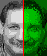
\includegraphics[scale=8.0]{imgs/gens_cmpl.png}
  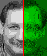
\includegraphics[scale=1.925]{imgs/dennis_cmpl.png}\\
  \vspace{-0.2cm}
  \captionof*{figure}{\fontsize{9pt}{10.8}\selectfont Figura 1. Compleição de imagem.}
\end{Figure}

\section*{Conclusions}

Obteve-se bons resultados em classificação em diferentes domínios, como classificação de dígitos,
identificação de objetos e reconhecimento de face. Em compleição, os algoritmos identificaram
de forma razoável características como nariz, olhos e boca no conjunto Olivetti. Todo código foi
documentado e disponibilizado de forma livre e gratuita como parte da biblioteca GoSPN\@.

\smallskip
\section*{References}
\vspace{0.1cm}

\AtNextBibliography{\fontsize{10pt}{12.0}\selectfont}
\printbibliography[heading=none]

\end{multicols*}

\end{document}
